\section{具体实现}
\subsection{CPU模块}
    CPU模块无可厚非是我们本次实现中最重要的一个模块,这个模块里面包含了非常多的原件,我们使用了如下组件来实现我们整个CPU。下面会一一列举。
\subsubsection{锁存单元}
    锁存单元包含if/id阶段,id/alu阶段,alu/mem阶段,mem/wb阶段四个大的锁存器,在上升沿触发。这几个锁存器的行为都受到中央控制单元的控制,中央控制单元可以命令其进行气泡的插入,以及重置功能。
    这四个部件的图以及具体信号如下。
% \usepackage{tabulary}

% \begin{tabulary}{0.7\textwidth}{|L|C|L|}
%     \hline
%     Short sentences      & \#  & Long sentences                                                 \\
%     \hline
%     This is short.       & 173 & This is much loooooooonger, because there are many more words.  \\
%     \hline
%     This is not shorter. & 317 & This is still loooooooonger, because there are many more words. \\
%     \hline
% \end{tabulary}  

\begin{center}
    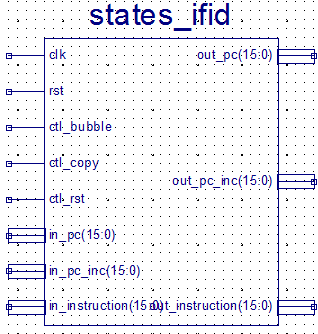
\includegraphics[height=10cm]{image/detail/detail_0.png}
    \fcaption{标题}

    \begin{tabular}{|p{3.5cm}|p{11cm}|}
        \hline 信号 & 信号描述 \\
        \hline clk & cpu的时钟信号,上升沿的时候根据ctl\_bubble和ctl\_rst进行控制。如果ctl\_bubble和ctl\_rst均为低电平则进行锁存,将in\_pc, in\_pc\_inc, in\_instruction进行锁存并输出。 \\
        \hline rst & 异步清空信号,由外部控制开关接入。 \\
        \hline ctl\_bubble & 气泡控制信号,由中央控制单元给出,如果该信号为高电平则表示下一个时钟上升沿,输出数据保持不变,低电平则该控制无效。 \\
        \hline ctl\_copy &  由中央控制单元给出,用来进行数据拷贝。\\
        \hline ctl\_rst & 重置控制信号,由中央控制单元给出,如果如果该信号为高电平则表示下一个时钟输出清空即为一条NOP指令,低电平则该控制无效。 \\
        \hline in\_pc & 表示下一条将要锁存的指令的pc。 \\
        \hline in\_pc\_inc & 表示下一条将要锁存的指令的pc+1。 \\
        \hline in\_instruction & 表示下一条将要锁存的指令内容 \\
        \hline out\_pc & 表示已经锁存的指令的pc。 \\
        \hline out\_pc\_inc & 表示已经锁存的指令的pc+1。 \\
        \hline out\_instruction & 表示已经锁存的指令。 \\
        \hline
    \end{tabular}

\end{center}
    

\subsubsection{PC锁存单元}
    PC锁存器,用来锁存PC,保证PC的改写受到中央控制部分的控制。我们规定在下降沿写入,组合逻辑输出。
    具体信号请看下表。